\documentclass[11pt,pdf,aspectratio=129]{beamer}
\usepackage{bibentry}
\usepackage{graphicx} % Allows including images
\usepackage{booktabs} % Allows the use of \toprule, 
\usepackage{array}
\usepackage{wrapfig}
\usepackage{graphics}
\usepackage{graphicx}
\usepackage{amsfonts}
\usepackage{amssymb}
\usepackage{amsthm}
\usepackage{textcomp}
% \usepackage{enumitem}
\usepackage{bibentry}
\usepackage{graphicx} % Allows including images
\usepackage{booktabs} % Allows the use of \toprule, 
% \usepackage[nottoc]{tocbibind}
\usepackage{threeparttable}
\usepackage{natbib}
\usepackage{mathrsfs}
\setlength{\parskip}{\baselineskip} 
\graphicspath{{./../Figures}}



\title{Checking HANK.}
\subtitle{Evidence from size-persistence tradeoff.}   
\author{\href{mailto://avlasov@nes.ru}{Vlasov Alexander}} 
\institute{NES}
\usetheme{Madrid}
% \usecolortheme{}

% \AtBeginSection{
% 	\begin{frame}
% 		\frametitle{Contents}
% 		\tableofcontents[currentsection]
% 	\end{frame}
% }

\begin{document}

\begin{frame}[fragile]
    \titlepage
\end{frame}


\section{Research question}



\begin{frame}\frametitle{Outcomes of \citet{KMV2018} model}
    \citet{KMV2018} HANK model outcomes:
    \begin{enumerate}
        \item Size-Persistence trade-off: Cumulative elasticity of aggregate consumption declines with the increase in autocorrelation of monetary shock in a nonlinear manner.
        \item Inflation-Output Tradeoff: the same Taylor rule shocks lead to the increased effects in Inflation-Output tradeoff.
    \end{enumerate}


  
\end{frame}


\begin{frame}\frametitle{Size-Persistence in RANK}
Rate path:
    \begin{equation*}
        r_t=\rho+e^{-\eta t}(r_0-\rho).\label{eq:InterestRatePath}
    \end{equation*}

NK policy    
\[C_0=\bar C\exp\left(-\frac{1}{\gamma}\int_0^\infty \left(r_s-\rho\right)\,ds\right).\]

Size:
\begin{equation*}
    R_0=\int_0^\infty \left(r_s-\rho\right)\,ds,\label{eq:KMVsize}
\end{equation*}


\[\frac{-d \log C_0}{dR_0}=\frac{1}{\gamma},\]


\end{frame}

\begin{frame}\frametitle{Picture of Size-Persistence trade-off}
    \begin{figure}\centering
        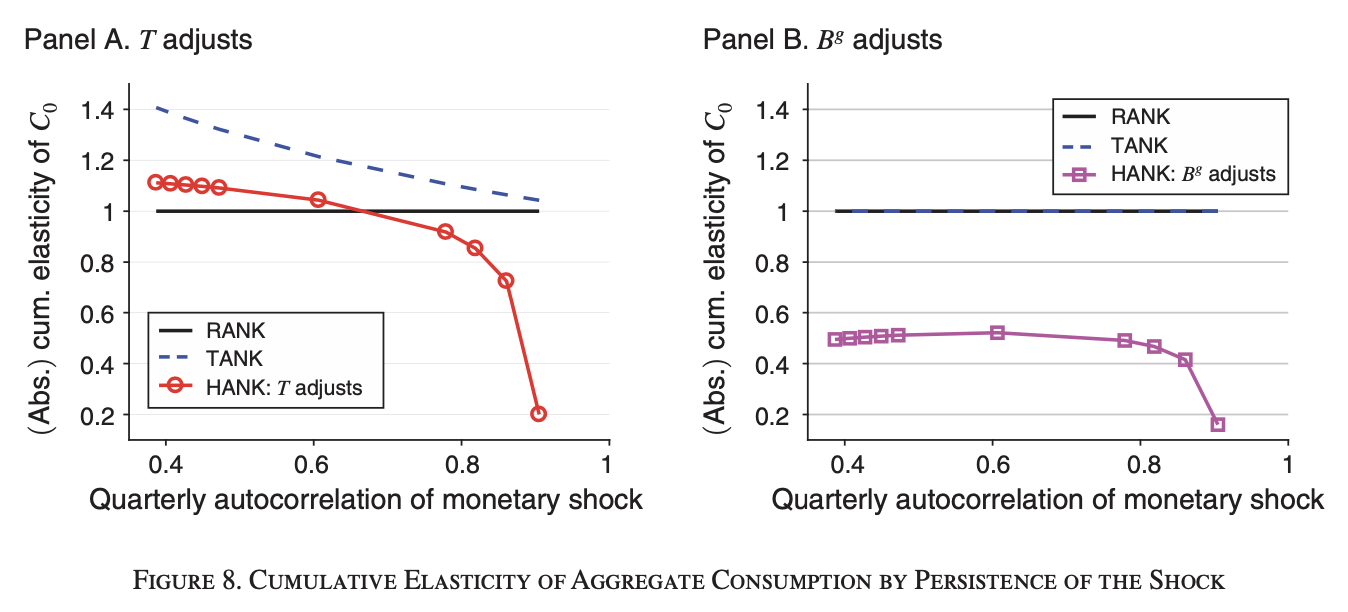
\includegraphics[scale=0.47]{Size_Persistence_KMV.png}
        \caption{The difference between the New Keynesian models from \citet{KMV2018}}
    \end{figure}
\end{frame}


\begin{frame}{Size-Persistent tradeoff by \citet{KMV2018}, formally}
    \begin{align}
        \textit{RANK:}&\quad& \frac{d}{d\nu}\frac{-d\log C_0}{dR_0}&=0     \label{eq:SizePersistenceRANK}\\
    \textit{TANK with $B^g$ adjustment:}&\quad& \frac{d}{d\nu}\frac{-d\log C_0}{dR_0}&= 0     \label{eq:SizePersistenceTANK_B}\\
    \textit{TANK with $T$ adjustment:}&\quad& \frac{d}{d\nu}\frac{-d\log C_0}{dR_0}&< 0     \label{eq:SizePersistenceTANK_T}\\
    \textit{HANK:}& \quad& 
        \frac{d^2}{d\nu ^2}\frac{-d\log C_0}{dR_0}&<0
        \label{eq:SizePersistenceHANK}
    \end{align}
    
\end{frame}


\begin{frame}\frametitle{Empirics Related to HANK}
% \begin{block}{Main work}
%     Model by \citet{KMV2018}
% \end{block}

\begin{block}{Microdata}
    \begin{itemize}
        \item \citet{HolmBlomhoff2021} find inconsistent Evidence of HANK -- the response is larger than generated by HANK.
    \end{itemize}
\end{block}
\begin{block}{MPC}
    \begin{itemize}
        \item  Estimation of MPC's\footnote{Actually MPB, but they argue that it doesn't affect the results} by \citet{Gross2020}:
        Increase of MPC is higher in 2008 than in 2011.
    \end{itemize}
\end{block}
\begin{block}{Heterogenity in Portfolios}
    \citet{Luetticke2021} find a heterogeneity in household portfolio responses to MP shocks.
\end{block}
\end{frame}


\section{Approach}

\begin{frame}\frametitle{Empirical approach:}
Based on method of \citet{HIM2023}.

I assume that the monetary policy rule is 
\[\left(r-r^*\right)_{t+h}=\tilde\phi_t\mathbb{E}\left[\pi_{t+1}\mid \mathcal{I}_t\right]+\varepsilon_t.\]
$\mathbb{E}_t\pi_{t+1}$ is the expectations of monetary authority about the inflation in quarter $t+1$.

I estimate the following State-Dependent LP-IV.
\begin{multline*}
    \left(r-r^*\right)_{t+h}=\alpha^h+\beta^h \hat\pi_t+\gamma^h \hat\pi_t\left(\mathit{Hawk}_{t}-\overline{\mathit{Hawk}}\right)\\ +\delta^h\left(\mathit{Hawk}_{t}-\overline{\mathit{Hawk}}\right)+\zeta^hZ+e_{t+h}^h,
\end{multline*}
\end{frame}

\begin{frame}{Empirical approach }

    \[\tilde \phi_{t+h}=\bar\phi+\phi_t=\hat \beta^h+\hat\gamma^h \left(\mathit{Hawk}_{t}-\overline{\mathit{Hawk}}\right).\]
    \[R_{0t}=\frac{1}{H}\sum_{h=1}^{H} \tilde \phi_{t+h}=\mathbb{E}_h \tilde \phi_{t+h}.\]
    \[\nu_t=\mathbb{E}_{h}\left[\left(\phi_{t+h}-\bar \phi\right)\left(\phi_{t+h-1}-\bar \phi\right)\right]\]

    \begin{align}
        \log \mathit{Consumption}&=\alpha_0+\alpha_1 R_0+\alpha_2\nu+\beta_1 R_0\nu \label{eq:linear}\\
        \log \mathit{Consumption}&=\alpha_0'+\alpha_1' R_0+\alpha_2'\nu+\beta_1' R_0\nu + \beta_2' R_0\nu^2\label{eq:quadratic}
    \end{align} 
\end{frame}






\section{Data}
\begin{frame}\frametitle{Data}
\begin{itemize}
        \item Natural rate of interest by \citet{HLW2017,HLW2023}
        \item Short-term rate ($r$) is by \citet{WuXia2016} and Fed Funds Rate 
        \item Consumption is U.S. Bureau of Economic Analysis``Real personal consumption expenditures per capita ''  (FRED A794RX0Q048SBEA) 
    \end{itemize}
\end{frame}

% \begin{frame}{Summary Statistics}
    
% \end{frame}




\section{Results}

\begin{frame}{Results: Monetary Shock Identification I}
    \begin{table}[ht] \centering \tiny
        \begin{threeparttable}
        \caption{Monetary Shock Identification.  First step} 
        \label{tab:Betas} 
      \begin{tabular}{@{\extracolsep{1pt}}lcccccc} 
        \\[-1.8ex]\hline 
        \hline \\[-1.8ex] 
         & \multicolumn{6}{c}{\textit{Dependent variable:}} \\ 
        \cline{2-7} 
        \\[-1.8ex] & DGS1 & DGS5 & DGS7 & DGS10 & DGS20 & DGS30 \\ 
        \\[-1.8ex] & (1) & (2) & (3) & (4) & (5) & (6)\\ 
        \hline \\[-1.8ex] 
         DGS2 & 0.727$^{***}$ & 1.029$^{***}$ & 0.921$^{***}$ & 0.743$^{***}$ & 0.316$^{**}$ & 0.202 \\ 
          & (0.071) & (0.090) & (0.110) & (0.112) & (0.127) & (0.130) \\ 
          & & & & & & \\ 
         Constant & $-$0.005$^{***}$ & $-$0.001 & $-$0.0002 & 0.0002 & $-$0.001 & $-$0.001 \\ 
          & (0.001) & (0.002) & (0.002) & (0.002) & (0.003) & (0.003) \\ 
          & & & & & & \\ 
        \hline \\[-1.8ex] 
        Observations & 382 & 382 & 382 & 382 & 382 & 382 \\ 
        R$^{2}$ & 0.634 & 0.766 & 0.666 & 0.583 & 0.327 & 0.206 \\ 
        Adjusted R$^{2}$ & 0.633 & 0.765 & 0.665 & 0.582 & 0.325 & 0.204 \\ 
        Res. Std. Error & 0.028 & 0.035 & 0.043 & 0.044 & 0.049 & 0.051 \\ 
        Wald test & 103.9$^{***}$&129.9$^{***}$& 70.49$^{***}$&43.71$^{***}$& 6.201$^{**}$&2.406\\
        Wu-Hausman& 3.699$^{*}$& 0.002&0.259&0.847& 9.345 $^{***}$ & 8.707$^{***}$\\
        \hline 
        \hline \\[-1.8ex] 
      \end{tabular} 
      \begin{tablenotes}[flushleft]
    \item\tiny{}This table reports first stage of \citet{BRW2021} monetary shock identification procedure for the FOMC announcement from 1994 to the most recent event 2021-04-28 (191 monetary events). OLS standard errors in the parenthesis. F-statistics on instrument insignificance is 44.030$^{***}$. Wu-Hausman stands for Hausman specification test for the endogeneity of a instrument $\left(\Delta R_{2,t}^{\textit{M}},-\Delta R_{2,t}^{\textit{NM}}\right)'$. $^{*}$p$<$0.1; $^{**}$p$<$0.05; $^{***}$p$<$0.01. 
      \end{tablenotes}
    \end{threeparttable}
      \end{table} 
      
\end{frame}



\begin{frame}{Results: Elasticity of consumprion}
    
\begin{table}[!htbp] \centering \tiny
    \begin{threeparttable}
    \caption{Elasticity of consumption to $(r-r^*)$.} 
    \label{tab:TotalElasticityofConsumption} 
  \begin{tabular}{@{\extracolsep{5pt}}lcc} 
  \\[-1.8ex]\hline 
  \hline \\[-1.8ex] 
   & \multicolumn{2}{c}{\textit{Dependent variable: $\log\,$Consumption}} \\ 
  \cline{2-3} 
  \\[-1.8ex] & \textit{OLS} & \textit{IV} \\ 
  \\[-1.8ex] & (1) & (2)\\ 
  \hline \\[-1.8ex] 
   $(r-r^*)$ & 0.092$^{***}$ & 0.197$^{***}$ \\ 
   & (0.008) & (0.013) \\ 
   & & \\ 
  Constant & 9.095$^{***}$ & 9.050$^{***}$ \\ 
   & (0.011) & (0.014) \\ 
   & & \\ 
 \hline \\[-1.8ex] 
 Observations & 361 & 361 \\ 
 R$^{2}$ & 0.255 & $-$0.079 \\ 
 Adjusted R$^{2}$ & 0.253 & $-$0.082 \\ 
 Residual Std. Error  & 0.207 & 0.249 \\ 
 F Statistic & 122.922$^{***}$& \\
  Weak instrument& &508.1$^{***}$\\
  Wu-Hausman & &622.3$^{***}$\\
  \hline 
  \hline \\[-1.8ex] 
  \end{tabular} 
  \begin{tablenotes}[flushleft]
\item\tiny This table reports the results of estimation of  consumption elasticity to the deviation of rate from its neutral (natural) value, $(r-r^*)$.  Weak instrument stands for first stage F-statisitic, that indicate, whether the $\hat{R}$ is a strong instrument.
Wu-Hausman stands for Hausman specification test for the endogeneity of a instrument  $\hat{R}$.
$^{*}$p$<$0.1; $^{**}$p$<$0.05; $^{***}$p$<$0.01  
  \end{tablenotes}
\end{threeparttable}
  \end{table} 

\end{frame}



\section{Conclusion}
\begin{frame}\frametitle{Conclusions}
    \begin{block}{So, should we believe in HANK?}

        The evidence above suggests that, we should. 
        At least we have found that consumption behaviour in size-persistent tradeoff corresponds to the HANK model.


    \end{block}
\end{frame}





%Thanks
\begin{frame}

\begin{center}
    \Large Place for your suggestions and comments!
\end{center} 
\begin{center}
    \footnotesize
If you have any other suggestions/comments  please write \href{mailto://avlasov@nes.ru}{avlasov@nes.ru}
\end{center}


\end{frame}



\begin{frame}[t, allowframebreaks]
    \frametitle{References}
   \bibliography{../misc/references.bib}
    \bibliographystyle{../misc/econ.bst}
    \end{frame}
\end{document}